
%(BEGIN_QUESTION)
% Copyright 2006, Tony R. Kuphaldt, released under the Creative Commons Attribution License (v 1.0)
% This means you may do almost anything with this work of mine, so long as you give me proper credit

En orifiseplate brukes til å måle strømningsraten av ultrarent vann i et farmasøytisk prosessanlegg, der vanlig enhet for væskestrøm er «liters per minute» (LPM). Beregn følgende parametere i denne flowmålesløyfen ved to ulike strømningsrater (78 LPM og 120 LPM):

$$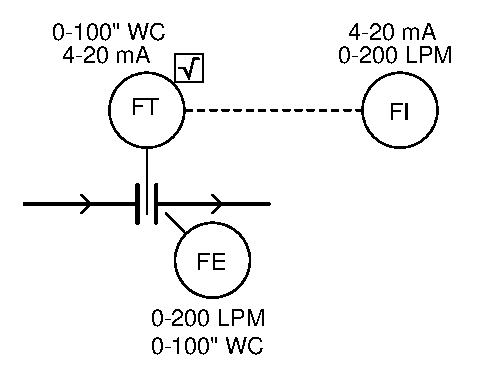
\includegraphics[width=15.5cm]{i00726x01.eps}$$

Merk at transmitteren har intern kvadratrotkarakterisering, slik at ingen ekstern kvadratrotutregner er nødvendig.

\begin{itemize}
\item {} {\bf Ved en strømningsrate på 78 LPM:}
\vskip 5pt
\item{} Orifiseplate $\Delta$P = \underbar{\hskip 50pt} " H$_{2}$O
\vskip 5pt
\item{} Utgangssignal fra differansetrykktransmitter = \underbar{\hskip 50pt} mA
\vskip 5pt
\item{} Avlesning på flowindikator = \underbar{\hskip 50pt} LPM
\end{itemize}

\vskip 10pt

\begin{itemize}
\item {} {\bf Ved en strømningsrate på 120 LPM:}
\vskip 5pt
\item{} Orifiseplate $\Delta$P = \underbar{\hskip 50pt} " H$_{2}$O
\vskip 5pt
\item{} Utgangssignal fra differansetrykktransmitter = \underbar{\hskip 50pt} mA
\vskip 5pt
\item{} Avlesning på flowindikator = \underbar{\hskip 50pt} LPM
\end{itemize}

\vskip 20pt \vbox{\hrule \hbox{\strut \vrule{} {\bf Forslag til sokratisk diskusjon} \vrule} \hrule}

\begin{itemize}
\item{} Et dårlig valg av flowmåler for akkurat denne applikasjonen ville være {\it magnetisk}. Forklar hvorfor.
\end{itemize}

\underbar{file i00726}
%(END_QUESTION)





%(BEGIN_ANSWER)

$$Q = k \sqrt{\Delta P}$$

Ved en volumetrisk strømningsrate på 200 liters per minute og et tilsvarende differansetrykk på 100 "WC, blir verdien av $k$ lik 20.

\begin{itemize}
\item {} {\bf Ved en strømningsrate på 78 LPM:}
\vskip 5pt
\item{} Orifiseplate $\Delta$P = \underbar{\bf 15.21} " H$_{2}$O
\vskip 5pt
\item{} Utgangssignal fra differansetrykktransmitter = \underbar{\bf 10.24} mA
\vskip 5pt
\item{} Avlesning på flowindikator = \underbar{\bf 78} LPM
\end{itemize}

\vskip 10pt

\begin{itemize}
\item {} {\bf Ved en strømningsrate på 120 LPM:}
\vskip 5pt
\item{} Orifiseplate $\Delta$P = \underbar{\bf 36} " H$_{2}$O
\vskip 5pt
\item{} Utgangssignal fra differansetrykktransmitter = \underbar{\bf 13.6} mA
\vskip 5pt
\item{} Avlesning på flowindikator = \underbar{\bf 120} LPM
\end{itemize}


%(END_ANSWER)





%(BEGIN_NOTES)



%INDEX% Måling, flow: beregninger i orifiseplatesløyfe

%(END_NOTES)


